\chapter[Método]{Método}

O método utilizado é uma interpretação do processo para descoberta de conhecimento proposto por \citeonline{fayyad1996data}, onde o objetivo principal é mapear um grande volume de dados para formas mais compactas, abstratas ou úteis para se encontrar padrões\footnote{O termo padrão é utilizado neste trabalho para designar um padrão encontrado nos dados.} e extrair informação.

A \autoref{fig:processo} apresenta o processo no qual, a partir de um conjunto de currículos Lattes, são obtidos indicadores em redes de coautoria inter- e intra-áreas que são analisados para determinar o impacto que uma área do conhecimento exerce em outra.

\begin{figure}[htpb]
  \centering
  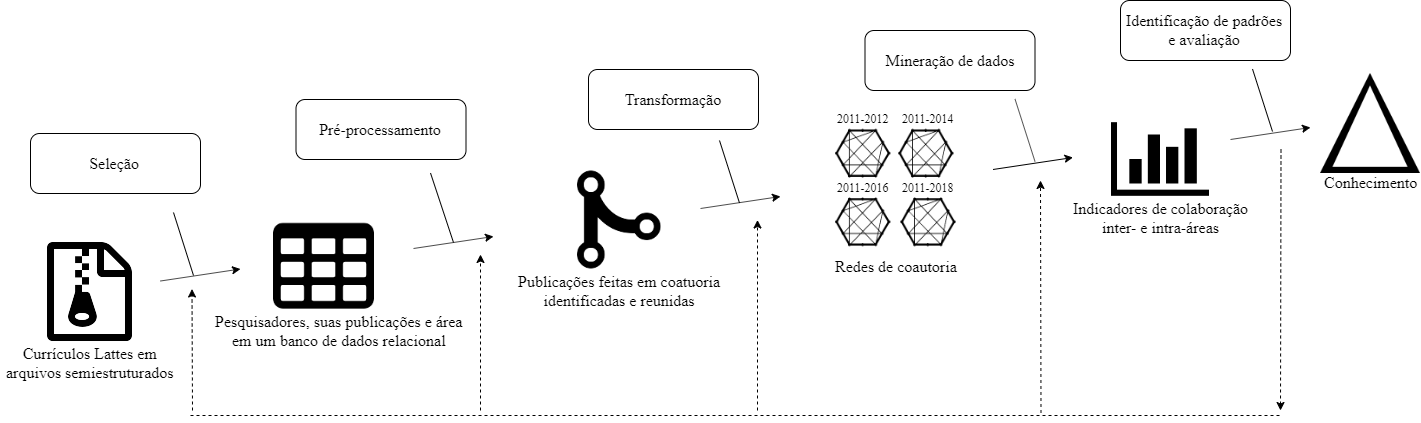
\includegraphics[width=1\textwidth]{figuras/metodo-diagrama-fayyad}
  \caption{Uma visão geral das etapas adotadas no processo de descoberta de conhecimento.}
  \label{fig:processo}
\end{figure}

As etapas de seleção, pré-processamento e transformação preparam o conjunto de dados para a etapa de mineração de dados, onde são aplicados algoritmos para extrair padrões. Esses padrões são então interpretados e utilizados para gerar conhecimento.

\section{Seleção}

Os currículos Lattes no formato XML foram processados por um sistema\footnote{Foram construídos dois programas. No primeiro, os atributos desejados do currículo são especificados, recuperados e armazenados intermediariamente em um arquivo no formato JSON. O segundo programa usa esse arquivo intermediário para fazer a carga nas tabelas do banco de dados remoto. Isso foi feito para evitar que a interpretação dos arquivos estivesse sujeita a instabilidades na conexão de rede e fosse possível continuar o processamento sem perdas em caso de falhas.} onde as áreas de atuação do pesquisador e sua produção bibliográfica foram extraídas e armazenadas em um banco de dados relacional.

A \autoref{fig:er} apresenta a modelagem de dados lógica do currículo centrada nos atributos que são de interesse para este trabalho, a qual descreve os pesquisadores atuando em múltiplas áreas do conhecimento e escrevendo múltiplas publicações científicas. O modelo físico do banco de dados está representado no \autoref{ap:diagramafisico}.

\begin{figure}[htpb]
  \centering
  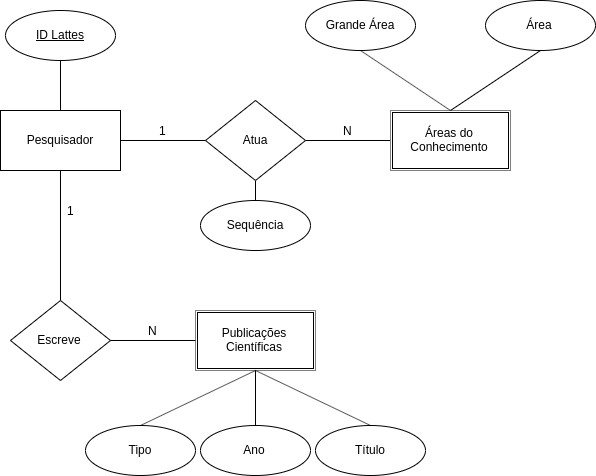
\includegraphics[scale=.5]{figuras/metodo-modelo-logico-lattes}
  \caption{Modelo entidade-relacionamento lógico descrevendo as relações entre o pesquisador, suas áreas de atuação e suas publicações científicas.}
  \label{fig:er}
\end{figure}

\section{Pré-processamento}

Os procedimentos para normalização do título das publicações e identificação da área de atuação do pesquisador são descritos nas subseções seguintes como parte da etapa de pré-processamento.

\subsection{Normalização do título das publicações}

Diversas produções científicas nessa área \cite{franceschet2011collaboration, mena2013prospecccao, reuther2006managing} descrevem casos onde uma publicação têm diversos nomes (sinônimos) e casos onde diferentes publicações possuem o mesmo nome (homônimos), cujos requerem tratamento a fim de obter um resultado mais confiável na etapa seguinte.

Publicações sinônimas acontecem neste trabalho porque os coautores não cadastraram o título da publicação exatamente da mesma maneira. Existem casos onde há abreviação de palavras, omissão de pontuação ou erros de digitação, por exemplo. Ainda, foram encontrados casos onde existem metadados para formatação do título, como itálico e negrito, que são colocados por alguns desses coautores.

Assim, o \autoref{alg:normalizacao} foi proposto para normalizar o título das publicações removendo diacríticos\footnote{Um diacrítico é um sinal gráfico que se coloca sobre, sob ou através de uma letra para alterar a sua realização fonética ou marcar qualquer outra característica linguística.}, espaços em branco e metadados de formatação ou qualquer outro elemento de marcação. Antes dessa etapa, podiam ser identificadas $1.230.082$ coautorias considerando o título exato e o ano da publicação. Após o pré-processamento, o número foi para $1.564.737$, o que já se traduz em uma melhora de $27$\% na identificação das coautorias.

\begin{algorithm}
\caption{Normalização do título das publicações}
\label{alg:normalizacao}
\begin{algorithmic}[1]
\Procedure{NormalizeTitulo}{titulo}
    \State $titulo \gets \Call{DesfazerHigienizacaoHtml}{titulo}$ \Comment{Codificação HTML-insegura}
    \If{$titulo$ contém o elemento CDATA}
        \State $titulo \gets$ conteúdo do CDATA 
    \EndIf
    \If{$titulo$ contém fragmentos que começam com $<$ e terminam com $>$}
        \State $titulo \gets titulo$ sem os fragmentos  
    \EndIf
    \State $titulo \gets \Call{NormalizeParaFormaNFKD}{titulo}$
    \State $resultado \gets \emptyset$
    \State $mantenhaDiacritico \gets Falso$
    \ForAll{$c \in titulo$}
        \If{$c$ não é branco \textbf{and} $c$ não é um diacrítico \textbf{or} $mantenhaDiacritico$}
            \State $resultado \gets resultado \cup \{c\}$
            \If{$c$ é um símbolo ASCII}
                \State $mantenhaDiacritico \gets Falso$
            \Else
                \State $mantenhaDiacritico \gets Verdadeiro$
            \EndIf
        \EndIf
    \EndFor
    \State $titulo\gets resultado$
    \State $titulo\gets \Call{NormalizeParaFormaNFKC}{titulo}$
    \State \Return $titulo$
\EndProcedure
\end{algorithmic}
\end{algorithm}

A normalização NFKD usada no método transforma uma cadeia de caracteres para a forma onde os diacríticos estão decompostos. Ainda, caracteres com o mesmo significado semântico são representados de uma única maneira. Com a normalização NFKC executada no final do procedimento, os diacríticos são recombinados usando regras canônicas.

Assume-se que publicações homônimas são mais difíceis de ocorrer dado que as coautorias serão identificadas apenas para publicações de um mesmo tipo em um mesmo ano, e por isso nenhum tratamento foi realizado. Porém, caso publicações homônimas existam nesse conjunto de dados, seria possível observar que a lista de coautores de um autor se dividiria em dois ou mais grupos altamente interconectados, sem colaborações entre os grupos diferentes \cite{franceschet2011collaboration}.

\subsection{Identificação da área de atuação do pesquisador}

As coautorias entre as áreas do conhecimento podem ser observadas se as áreas do conhecimento na qual o pesquisador atua estão disponíveis. Entretanto, nem sempre todas as áreas do conhecimento listadas estão relacionadas à sua produção científica. Existem casos onde professores, por exemplo, adicionam Educação às suas áreas de atuação sem terem desenvolvido publicações científicas na área.

O procedimento descrito pelo \autoref{alg:identificacaoarea} assume que existe uma área do conhecimento na qual o pesquisador mais se encaixa, e esta seria a área do conhecimento mais frequente dentro da grande área que mais vezes aparece no currículo. Em casos de empate, a área que aparecer primeiro no currículo será selecionada, dado que o método de ordenação é estável.

\begin{algorithm}
\caption{Identificação da área de atuação do pesquisador}
\label{alg:identificacaoarea}
\begin{algorithmic}[1]
\Require{$A$ é o conjunto de áreas de atuação do pesquisador declaradas no currículo}
\Ensure{Nome da área do conhecimento identificada para o pesquisador}
\Procedure{IdentificaArea}{A}
    \State $areaSelecionada \gets \textbf{nulo}$
    \State $raiz \gets \Call{NoVazio}$
    \ForAll{$area \in A$}
        \State $nomeGrandeArea \gets \Call{NomeGrandeArea}{area}$
        \State $nomeArea \gets \Call{NomeArea}{area}$
        \State $no \gets \Call{RecuperaNo}{raiz, nomeGrandeArea}$
        \If {$no$ não existe}
            \State $no \gets \Call{IncluirNo}{raiz, nomeGrandeArea}$
        \EndIf
        \State $no.contagem++$
        \If{$nomeArea$ está preenchida}
            \State $folha \gets \Call{RecuperaNo}{no, nomeArea}$
            \If{$folha$ não existe}
                \State $folha \gets \Call{IncluirNo}{no, nomeArea}$
            \EndIf
            \State $folha.contagem++$
        \Else
            \State $no.contagemVazios++$
        \EndIf
    \EndFor
    \State $N \gets \Call{OrdenaPorContagem}{raiz.filhos, \textbf{decrescente}}$
    \While{$areaSelecionada \neq \textbf{nulo}$}
        \State $no \gets \Call{Proximo}{N}$
        \If{$no.contagem \neq no.contagemVazios$}
            \State $F \gets \Call{OrdenaPorContagem}{no.filhos, \textbf{decrescente}}$
            \State $areaSelecionada \gets \Call{Proximo}{F}$
        \EndIf
    \EndWhile
    \State \Return $areaSelecionada$
\EndProcedure
\end{algorithmic}
\end{algorithm}

\section{Transformação}

A partir das publicações científicas obtidas nos currículos é possível identificar dois pesquisadores como coautores se uma mesma publicação aparece em seus currículos. Com isso é possível construir uma rede de coautoria onde os nós são pesquisadores e os vértices a coautoria entre eles.

O \autoref{alg:coautoria} foi proposto para construir a lista de adjacência identificando duas publicações como coautorias se os títulos são pelo menos uma porcentagem similares. Sabendo que uma coautoria só deve ser identificada se as publicações forem do mesmo tipo e ano, apenas publicações com essas características devem ser fornecidas para a execução procedimento.

\begin{algorithm}
\caption{Identificação de coautorias}
\label{alg:coautoria}
\begin{algorithmic}[1]
\Require{$P$ é o conjunto de publicações de um dado ano e $sim$ a similaridade mínima para aceitar publicações como sendo sinônimas}
\Ensure{$C$ é a lista de adjacência da coautoria de publicações}
\Procedure{IdentificaCoautoria}{$P, sim$}
    \State $C\gets \emptyset$
    \For{$i\gets 1 \textbf{ to } |P|$}
        \For{$j\gets i \textbf{ to } |P|$}
            \State $a_1 \gets P[i].autor$
            \State $a_2 \gets P[j].autor$
            \State $p_1 \gets P[i].palavras$
            \State $p_2 \gets P[j].palavras$
            \State $t_1 \gets P[i].titulo$
            \State $t_2 \gets P[j].titulo$
            \State $sim_{tam}\gets \dfrac{\min\{|t_1|, |t_2|\}}{\max\{|t_1|, |t_2|\}}$
            \If{$a_1 \neq a_2\textbf{ and } |p_1| \geq 3 \textbf{ and } |p_2| \geq 3 \textbf{ and } sim_{tam} \geq sim$}
                \State $dist\gets \Call{DistanciaLevenshtein}{t_1, t_2}$
                \State $sim_{lev}\gets 1 - \dfrac{dist}{\max\{|t_1|, |t_2|\}}$
                \If{$sim_{lev} \geq sim$}
                    \State $C\gets C\cup\{(P[i], P[j])\}$
                \EndIf
            \EndIf
        \EndFor
    \EndFor
    \State $C\gets \Call{TransformaComponentesConexasEmCliques}{C}$
    \State \Return $C$
\EndProcedure
\end{algorithmic}
\end{algorithm}

Assim, em um conjunto de publicações do mesmo tipo e ano, podem ser identificadas como coautorias as publicações com títulos que são, por exemplo, pelo menos $90$\% similares, pertencem a autores diferentes e os títulos contêm pelo menos duas palavras. O cálculo da similaridade é feito a partir da distância de Levenshtein \cite{levenshtein1965binary}, que quantifica a dissimilaridade entre os títulos. A transformação das componentes conexas em cliques no final do procedimento garante que todos os coautores estejam relacionados entre si, uma vez que isso garante que para cada publicação todas as coautorias são mútuas.

Em consequência disso, o número de coautorias identificadas aumenta consideravelmente. O gráfico da \autoref{fig:composicaocoautorias} mostra a composição das coautorias identificadas em termos da similaridade quando os títulos podem ser 90\% similares, indicando que quase $1/4$ das coautorias foram identificas pelo procedimento aplicado. Os casos de coautorias identificadas pela transformação das componentes conexas em cliques não estão retratadas no gráfico, mas somam $164.876$ coautorias que não seriam identificadas.

\begin{figure}[htpb]
  \centering
  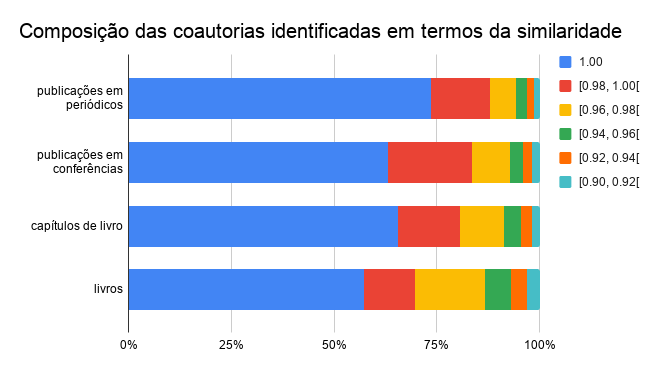
\includegraphics[scale=.5]{figuras/metodo-composicao-coautorias}
  \caption{Composição das coautorias identificadas em termos da similaridade quando os títulos podem ser 90\% similares.}
  \label{fig:composicaocoautorias}
\end{figure}

\section{Mineração de dados}

A partir das redes de coautoria foi construída a rede apresentada na \autoref{fig:grafocolaboracao}, que descreve como as coautorias acontecem entre as áreas do conhecimento. Isso foi possível atribuindo as coautorias de um pesquisador à área identificada pelo \autoref{alg:identificacaoarea}, excluindo as coautorias feitas intra-área.

O mapa de calor das coautorias entre as áreas exposto na \autoref{fig:mapadecalorcolaboracao} foi gerado pela matriz de adjacência da rede de coautoria entre as áreas do conhecimento, onde cada linha da matriz foi normalizada pela estratégia de máximos e mínimos. Assim, o valor 1 na linha representa o esforço máximo exercido na colaboração e o valor 1 na coluna representa esforço percebido na colaboração.

Esse mapa de calor possibilitou gerar uma matriz de adjacência bastante interessante, de onde foi possível construir o dígrafo de impacto representado na \autoref{fig:grafoimpacto}. Nele, apenas o esforço máximo recebido na colaboração é considerado para construir a lista de adjacência, onde o nó de origem é o rótulo da coluna e o nó de destino é o rótulo da linha.

\section{Identificação de padrões e avaliação}

Foram utilizados gráficos de segmento, histogramas, mapas de calor, tabelas, grafos e dígrafos para ler e visualizar os resultados. Uma vez que existiam dados faltantes, foi realizada a análise condicional. Ainda, o resultado de outros artigos foram avaliados para verificar o que era observado.

Ao avaliar resultados, as etapas anteriores foram revisitadas com o intuito de aprimorar o tratamento dos dados. As etapas de seleção, pré-processamento e mineração de dados foram revisitadas múltiplas vezes. O mapa gerado na etapa de mineração, por exemplo, foi gerado apenas nas últimas iterações.
